\documentclass[00-main.tex]{subfiles}

\begin{document}

\section{Application to Rat Decision Making}\label{sec:applications}

\subsection{Dataset Description}
To illustrate application to empirical data, we applied this method to behavioral data from a self-paced, two-alternative forced-choice (2AFC) reaction time task performed by rats, as detailed in \citet{reinagel_speed_2013}. In this experimental paradigm, rats had continuous, 24-hour access to the task from their home cages. Trials were self-initiated via a central start port, triggering a visual stimulus of 100 white dots. A subset of these dots moved coherently toward the left or right (signal), while the remainder moved randomly (noise). Rats viewed the stimulus freely until licking a left or right response port to register their choice, which immediately terminated the stimulus. Correct responses yielded a water reward while error responses resulted in a very small reward.

To isolate intrinsic temporal variability of decision-making parameters from experimentally-induced variability, a contiguous sequence of $n=$42,840 trials was selected from a single rat (ID 195) over a 100-day period, starting after that rat had reached the criterion of 80\% correct performance on the task. This sequence was chosen because it demonstrates the nonstationarities and temporal correlations that the proposed method is designed to address, as illustrated below in Figure~\ref{fig:rat-beh}, and is publicly available on Dryad \citep{reinagel_rat_2026}. Throughout this sequence, task difficulty was held constant at 85\% motion coherence, with the direction of motion chosen randomly to be leftward or rightward on each trial.\footnote{There were two experimentally imposed one-trial-back sequential dependencies: rewards following correct trials were larger than rewards following error trials, and correction trials were imposed after some errors.} Consequently, most observed fluctuations in decision behavior are attributable to the passage of time and internal state changes rather than external manipulations. For the $i^{th}$ trial, stimulus coherence is encoded as the signed covariate $X_i \in \{-0.85, +0.85\}$ (negative for leftward, positive for rightward motion), and the decision outcome as the signed reaction time $Y_i$ (negative for leftward, positive for rightward choice). Here, the drift rate is modeled as a linear function of coherence $v_i = \beta_v X_i$, so $\beta_v$ estimates are reported instead of $v$ throughout these analyses. With the experimental conditions held constant, we looked for evidence of DDM parameters varying systematically over time, across both within-day and between-day timescales.

\newpage

\subsection{Descriptive Data Analysis}
\subsubsection{Choices and Reaction Times Reveal Nonstationary Decision Behavior}
\emph{Between-day} temporal structure shows this rat typically started performing trials after 18:00, continued vigorously for a few hours, and then performed additional bouts over the course of the night (Figure~\ref{fig:rat-beh}A). Vertical breaks in the heatmap were self-initiated by the rat, while horizontal breaks were experimentally initiated, i.e., the rat was temporarily removed from the task. Over the 100 days, this rat gradually performed fewer and fewer trials per day, a trend explained only by calendar day and no other measured covariates that we checked. Accuracies fluctuated during the first 35 days, showing a gradual increase before plateauing, indicative of improvement with practice; likewise, reaction times were highly variable during these days. From day 36 onward, accuracies continued to fluctuate day-to-day, but less so, and reaction times gradually decreased (Figure~\ref{fig:rat-beh}C). After the practice period, reaction times showed positive autocorrelation at one- and two-day lags; accuracy autocorrelations were not distinguishable from zero (95\% pointwise intervals).

\emph{Within-day} cumulative reward increases in proportion to the number of trials performed so far (Figure~\ref{fig:rat-beh}B, upper); therefore, effects of trial-in-day could be explained in part by reward satiety. The rat performed at least 100 trials on every day tested, exceeded 500 trials on half the days, and rarely completed 800 trials in a day. Therefore, the sampling (number of observed trials pooled across days) declined with trial-in-day (Figure~\ref{fig:rat-beh}B, lower). In the first 20 trials of each day, the rat was less accurate and responded more quickly. We speculate that this could be transiently unregulated behavior due to intense thirst, alleviated after a few drops of water were earned. Thereafter, accuracies stabilized but reaction times continued to increase (Figure~\ref{fig:rat-beh}D). Autocorrelations decayed to zero quickly, indicating that fitting the trends with splines accounted for much of the trial-to-trial dependence.

These patterns motivate modeling systematic parameter changes and accounting for remaining temporal dependence in uncertainty estimates.

\begin{figure}[H]
    \centering
    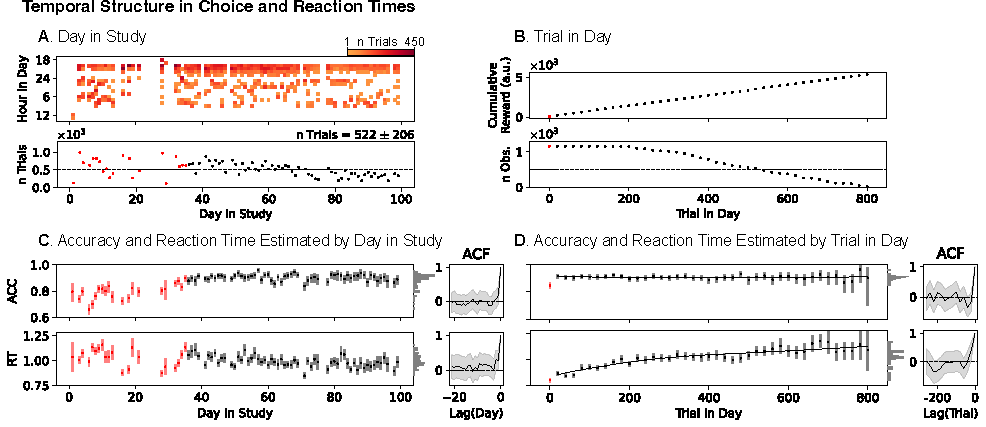
\includegraphics[width=1\textwidth]{docs/manuscript/figures/fig05-rat195.pdf}
    \caption{\emph{Choices and Reaction Times Reveal Nonstationary Decision Behavior.}}
    \subcaption*{
    Behavioral results are displayed for $n$=42,840 random dot motion discrimination trials performed by a single rat over 100 days, beginning after the rat had reached the criterion of 80\% correct performance on the task. Left column (A, C) shows between-day temporal structure; right column (B, D) shows within-day temporal structure. A ``day'' is defined as the 24-hour period beginning at 18:00, which was around the time of day this rat usually chose to start trials. Panels A and C exclude the first 20 trials of each day; panels B and D pool days after day 35 and 20-trial bins labeled 0--800. (A; top) Trial heat map showing trial counts per hour (colormap). (A; bottom) Points show trial counts per day ($n = 522 \pm 206$; mean $\pm$ SD across 79 observed days). Points in red in A and C (the first 35 days) indicate a period in which the rat continued to improve with practice, before stabilizing thereafter. (B; top) Non-overlapping bins of 20 trials within a day were pooled across days. Points indicate the cumulative water reward received per trial bin, averaged over days. (B; bottom) Points show number of observations (trials) contributing to each point estimate in Panel D. Points in red in B and D (the first 20 trials of each day) are distinguished because accuracy was notably lower in this bin. (C,D) Estimated accuracies and reaction times, with error bars denoting 95\% confidence intervals assuming $iid$ trials, and either a binomial sampling distribution (for accuracy) or a normal approximation to the sampling distribution (for RT). Insets to the right display autocorrelation functions (ACFs) with 95\% pointwise confidence intervals, assuming stationarity. The practice period (red points in C) and first 20 trials of the day (red point in D) were excluded from the ACFs, as they appear nonstationary. Within-day trends in (D) were modeled by fitting piecewise quadratic splines (curves) and then the ACFs were computed on the residuals.
    }
    \label{fig:rat-beh}
\end{figure}

\subsubsection{DDM Parameters Reveal Nonstationary Decision States}
\emph{Between-day} temporal structure in DDM parameters estimated by day paralleled the behavior, in which parameters fluctuated widely during the initial practice period before stabilizing (Figure~\ref{fig:rat-ddm}A, C). In principle, the observed changes in reaction times (Figure~\ref{fig:rat-beh}C) could reflect changes in $a$, $\beta_v$, $z$, or some combination thereof. Fitting the DDM by day reveals that, in this case, they are explained by both increases in the decision boundary ($a$) and drift rate coefficient ($\beta_v$), suggesting the rat became both more cautious and attentive to the motion stimulus with practice. The rat also had a persistent rightward bias (positive $z$) that was strongest at the start of the study and decreased thereafter. All panels show estimates from the proposed pseudo-MLE with confidence intervals \eqref{eq:V_ar} robust to misspecification and temporal dependence, as assessed in Section~\ref{sec:simulations}. Comparing Figure~\ref{fig:rat-ddm} Panels (A) and (C), the latter controlling for within-day nonstationarity by including trial-in-day spline covariates and reporting each day's fitted value at the reference trial 400, yielded broadly similar between-day point estimates. Confidence intervals in (C) were similar in width to those in (A); standard errors were on average 1.35\% smaller, averaging relative reductions across days and parameters. The simulations in Section~\ref{sec:simulations} show improved uncertainty estimates under unmodeled variability and temporal dependence, with some finite-sample bias. Thus, accounting for within-day nonstationarity yielded little change in uncertainty, without notably altering the inferred between-day fluctuations. After the practice period, both daily analyses showed positive lag-one autocorrelation in boundary height and starting point, but no detectable autocorrelation in non-decision time (95\% pointwise intervals).

\emph{Within-day} temporal structure in DDM parameters estimated by trial-in-day likewise paralleled the behavior, where the low accuracy and fast reaction times in the first 20 trials of each day (Figure~\ref{fig:rat-beh}D) were explained by a low decision boundary ($a$) and drift rate coefficient ($\beta_v$; Figure~\ref{fig:rat-ddm}B). The monotonic increase in reaction times throughout the day (Figure~\ref{fig:rat-beh}D, lower) was accompanied by overall increases in the decision boundary ($a$) and non-decision time ($t_0$), and a decrease in the drift rate coefficient ($\beta_v$), most apparent in Figure~\ref{fig:rat-ddm}D. This suggests the rat became more cautious and less eager as the day progressed as its need for water was gradually satiated. In (D), the drift rate coefficient ($\beta_v$) decreased across the day, whereas fluctuations in the relative starting point ($z$) were not distinguishable from a constant at this confidence level, highlighting the importance of uncertainty quantification for avoiding misinterpretation of parameter fluctuations. Collectively, the observed trends in DDM parameters reflected changes in latent decision states, especially the overall increases in decision bound and non-decision time within a day. These changes are large relative to their uncertainty, indicating that the observed changes in decision states reflect nonstationarity rather than estimation noise.

\begin{figure}[H]
    \centering
    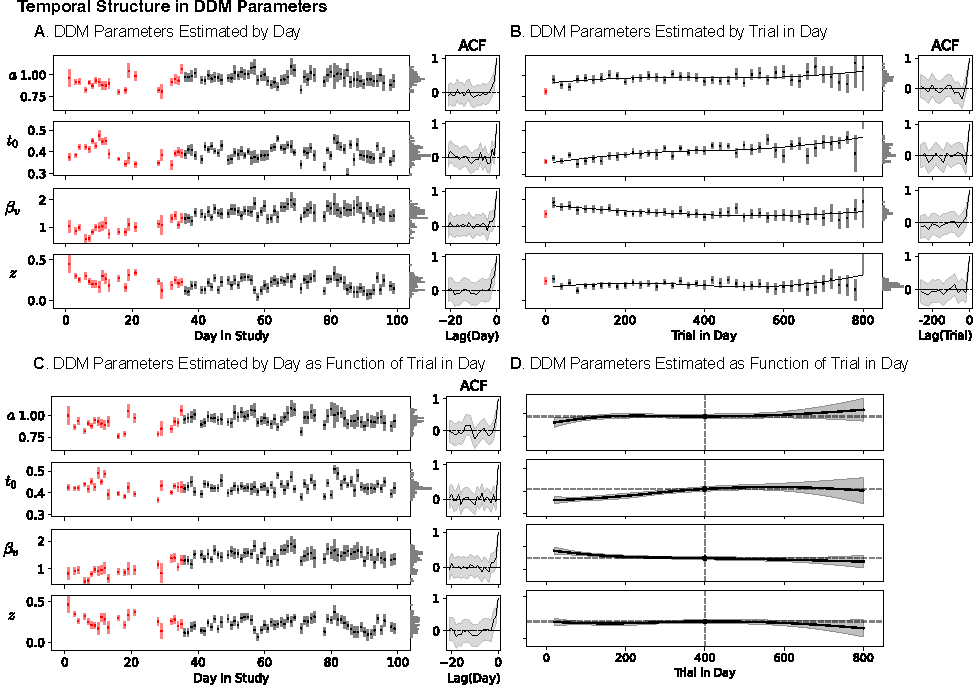
\includegraphics[width=1\textwidth]{docs/manuscript/figures/fig06-rat195.pdf}
    \caption{\emph{DDM Parameters Reveal Nonstationary Decision States.}}
    \subcaption*{
        Estimated DDM parameters and coefficient $\beta_v$ of motion coherence, corresponding to Figure~\ref{fig:rat-beh}. All panels show pseudo-MLE estimates with 95\% confidence intervals \eqref{eq:V_ar} robust to temporal dependence and parameter variability. Left column (A, C) shows between-day structure; right column (B, D) shows within-day structure. (A) Daily parameter/coefficient estimates, excluding the first 20 trials of each day; red marks the practice period, excluded from the between-day ACF insets. (B) Parameter/coefficient estimates per 20-trial bin within a day, pooled over days after day 35, and piecewise quadratic splines fit to point estimates; red marks the first 20 trials, excluded from the residual ACF insets. (C, D) Extended analyses accounting for within-day nonstationarity omitted from (A, B). (D) A single model is fit to trials after day 35 in 20-trial bins labeled 20--800, excluding the first 20 trials of each day, with parameters modeled as piecewise quadratic splines of the trial-in-day covariate. Simultaneous 95\% confidence bands are obtained via the delta method applied to \eqref{eq:V_ar}, with a Bonferroni correction over the number of unique trial bins per day. Vertical dashed lines mark reference trial 400; horizontal dashed lines show the corresponding reference values. (C) Extends the between-day analysis of (A) by holding all spline shape coefficients fixed at the values estimated in (D), refitting only the intercept per day, and reporting the fitted value at the reference trial 400, thereby isolating between-day shifts in each DDM parameter while controlling for within-day nonstationarity. Confidence intervals in (C) are conditional on the estimated spline shape coefficients.
    }
    \label{fig:rat-ddm}
\end{figure}
\end{document}
